
%! Author = lili
%! Date = 6/9/26

% 76-83: Genetik der Geschlechtsbestimmung I + Analyse von Familienstammbäumen komplett
%% https://link.springer.com/chapter/10.1007/978-3-662-70442-4_11

% 188-202: Genmutationen komplett
%% https://link.springer.com/chapter/10.1007/978-3-662-70442-4_6

% bis F 6 ist wdh

% \section{Extrachromosomale Gene}

\section{Geschlechtschromosomen}\label{sec:geschlechtschromosomen}

% TODO F  8 - 13, 17 - 21

\subsection{\gls{x_chromosom} Inaktivierung bei Säugern}\label{subsec:x-chromosom-inaktivierung-bei-saugern}
% TODO F 14 - 16

\subsection{Aneuploidie-Syndrome}\label{subsec:aneuploidie-syndrome}
\defin{aneuploidie}
Syndrome sind:
\begin{mytable}
    \begin{tabular}{ p{2cm} p{2cm} p{2cm} p{2cm} p{7cm} }
        \textbf{Syndrom} & \textbf{Geschlecht} & \textbf{Karyotyp} & \textbf{Häufigkeit} & \textbf{Merkmale} \\
        Turner-Syndrom (UTS)
        & weiblich
        & 45, X0
        & 1/2500
        & Kleinwuchs (ca.
        1,5 m), kurzer Hals, Östrogenmangel (therapierbar), unfruchtbar, mögliche Missbildungen innerer Organe \\

        Klinefelter-Syndrom
        & männlich
        & 47, XXY
        & 1/660
        & sehr großer Körper (>1,8 m), keine Spermienbildung, unfruchtbar, oft nicht diagnostiziert, erhöhte Neigung zu Diabetes \\

        Triplo-X-Syndrom
        & weiblich
        & 47, XXX
        & 1/1000
        & äußerlich unauffällig, normale Pubertätsentwicklung, meist fruchtbar \\

        Diplo-Y-Syndrom
        & männlich
        & 47, XYY
        & 1/590
        & etwas überdurchschnittliche Körpergröße, normale Pubertät, fruchtbar, Verhalten unauffällig
    \end{tabular}
    \caption{Chromosomenaberrationen der Geschlechtschromosomen und ihre Merkmale \cite{vorlesung12}}
\end{mytable}

\begin{fr}
    \textbf{Gibt es ``X0'' nicht schon in normalen weiblichen Säugern, weil das zweite X
    inaktiviert ist? Bei ``inaktiviertem X'' gibt es auch kein Y, also sollte ``X0'' einen normalen
    weiblichen Organismus ergeben.}
    Nicht alle Gene auf dem \gls{x_chromosom} werden inaktiviert.
    Einige Gene entkommen der X-Inaktivierung: sogenannte Escape-Gene.

    Beim Turner-Syndrom (X0) entsteht der Krankheitsmechanismus dadurch, dass nicht alle Gene des zweiten \gls{x_chromosom}s durch die X-Inaktivierung abgeschaltet werden.
    Einige sogenannte Escape-Gene bleiben aktiv, sodass Frauen mit XX normalerweise zwei aktive Kopien dieser Gene besitzen.
    Fehlt beim X0-Karyotyp das zweite \gls{x_chromosom}, liegt von diesen Genen nur eine Kopie vor.
    Dadurch entsteht ein Mangel an Genprodukten, was als Haploinsuffizienz bezeichnet wird und zu den typischen Merkmalen des Turner-Syndroms führen kann.
\end{fr}

% F 22 - 25, 30 - 32
\subsubsection*{Trisomie 21}
\begin{itemize}
    \item Down-Syndrom
    \item in ``jeder'' Zelle 47 \gls{chromosom}en statt 46 vorhanden
    \item \gls{chromosom} 21 dreimal statt zweimal vorhanden (95\% der Fälle)
    \item Translokations-Trisomie 21: Angeheftet meist an 13, 14, 15 oder 22 (5\%)
    \item mit etwa 1/650 Geburten die häufigste \gls{chromosomen_abberation}
    \item Risiko abhängig von Alter der Mutter
\end{itemize}~\cite{vorlesung12}
% TODO Allg. Genetik 13.3 Numerische und strukturelle Chromosomenaberrationen
% TODO F 31 / 32 Diagnose von Aneuploidien

\subsubsection{Nondisjuktion}
% F 26 - 28
\defin{nondisjunction}
\begin{figure}[H]
    \centering
    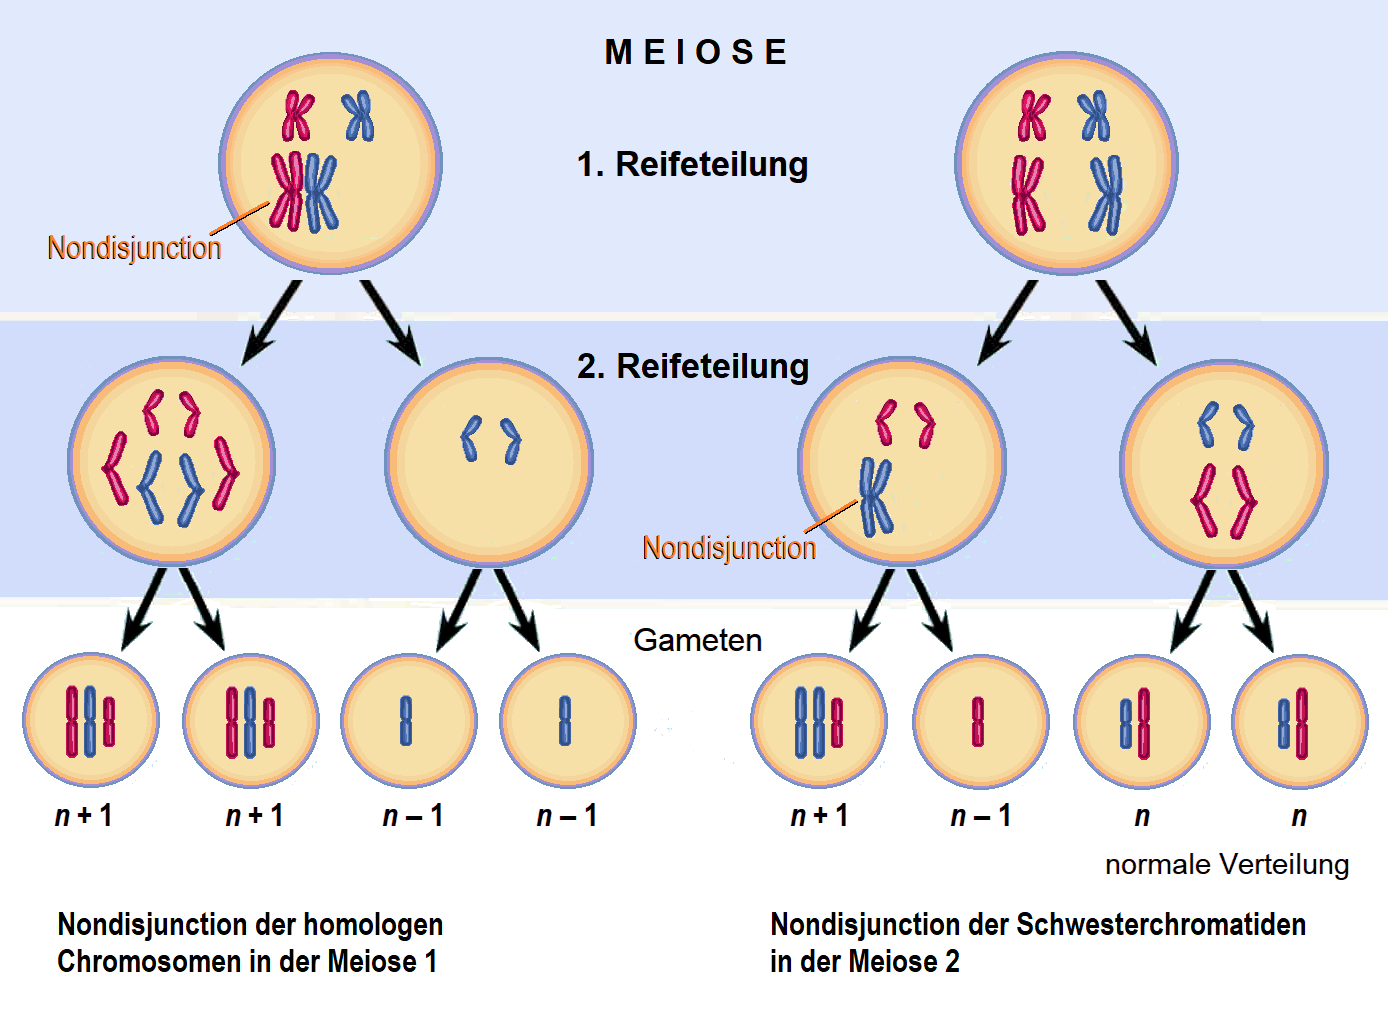
\includegraphics[width=\linewidth]{bilder/nondisjunction}\label{fig:figure24}
\end{figure}
\verb|https://de.wikipedia.org/wiki/Non-Disjunction#/media/Datei:Non-Disjunction_de.png|

\section{Konvention zur Darstellung von Erbgängen}\label{sec:konvention-zur-darstellung-von-erbgangen}
\begin{itemize}
    \item Männliche Personen werden durch Quadrate dargestellt.
    \item Weibliche Personen werden durch Kreise dargestellt.
    \item Die Nachkommen (Geschwister) von links nach rechts jünger.
    \item Homozygot gesunde Personen erhalten offene Symbole.
    \item Homozygot kranke Personen erhalten ausgefüllte Symbole.
    \item Heterozygote werden durch halbgefüllte Symbole gekennzeichnet.
\end{itemize}
% TODO karteikarte

% TODO Beispiel

\section{Mutationen}\label{sec:mutationen2}
Mögliche Ursachen von Mutationen sind:
\defin{basale_mutationsrate}
\defin{spontane_mutation}
\defin{induzierte_mutation}
Es können Veränderungen innerhalb eines Gens auftreten (Genmutationen) oder einzelne Basen ausgetauscht werden (siehe \gls{snp}). Chromosomen-Mutationen und -Aberrationen sind größere Veränderungen der DNA-Struktur.
Es gibt Reparatursysteme zum Reparieren von Mutationen. \cite{vorlesung12}
%  F 37 - 47 (40-42 sind Übergang)
% TODO F 44+45?
\begin{figure}[H]
    \centering
    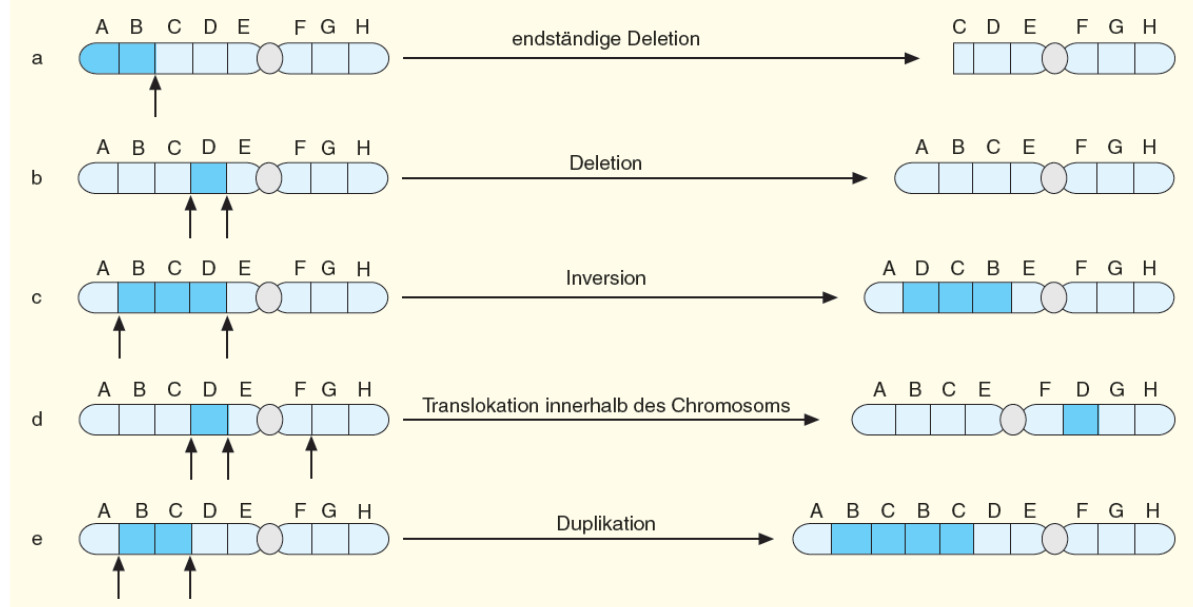
\includegraphics[width=\linewidth]{bilder/mutationen}\label{fig:figure23}
\end{figure}~\zitat{Unter strukturellen Chromosomenaberrationen versteht man ganz allgemein
dauerhafte Veränderungen der linearen Abfolge der Gene auf den
Chromosomen: Es können z.B. Chromosomenstücke fehlen (synonym: \textbf{Defizienz} oder \textbf{Deletion}), verdoppelt vorliegen \textbf{(Duplikation)}, mit umgekehrter Genfolge im Chromosom eingebaut \textbf{(Inversion)} oder zwischen nicht‐homologen Chromosomen ausgetauscht sein \textbf{(Translokation)}.
 An der Entstehung von Chromosomenmutationen sind wohl immer
Chromosomenbrüche beteiligt, die oftmals als Konsequenz einer defekten
Beendigung der Replikation auftreten.}{\cite{Knust2025_Mutationen}}

\begin{figure}[H]
    \begin{subfigure}[t]{0.33\textwidth}
        \centering
        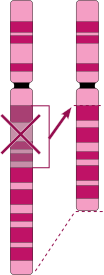
\includegraphics[width=\linewidth]{bilder/deletion}
        \caption{Deletion}
    \end{subfigure}
    \hfill
    \begin{subfigure}[t]{0.33\textwidth}
        \centering
        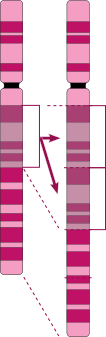
\includegraphics[width=\linewidth]{bilder/duplikation}
        \caption{Duplikation}
    \end{subfigure}
    \hfill
    \begin{subfigure}[t]{0.33\textwidth}
        \centering
        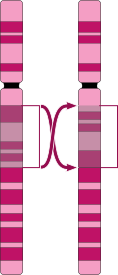
\includegraphics[width=\linewidth]{bilder/inversion}
        \caption{Inversion}
    \end{subfigure}
    \caption{Mutationen, die ein Chromosom betreffen.}\label{fig:figure22}
\end{figure}

\begin{figure}[H]
    \begin{subfigure}[t]{0.45\textwidth}
        \centering
        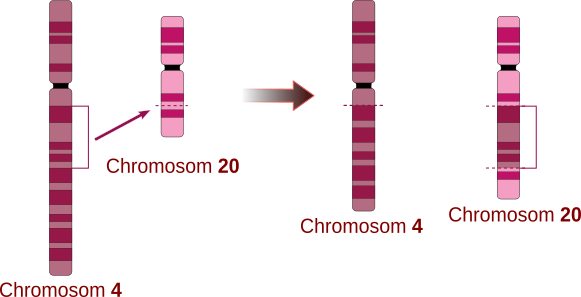
\includegraphics[width=\linewidth]{bilder/insertion}
        \caption{Insertion}
    \end{subfigure}
    \hfill
    \begin{subfigure}[t]{0.45\textwidth}
        \centering
        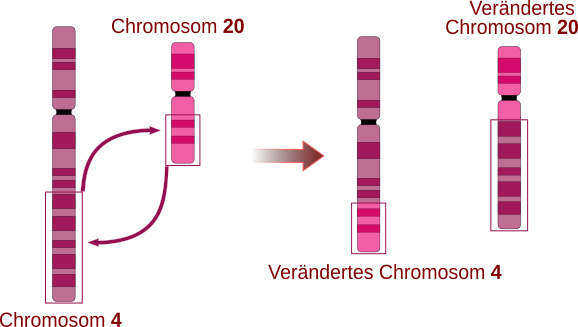
\includegraphics[width=\linewidth]{bilder/translokation}
        \caption{Translokation}
    \end{subfigure}
    \caption{Mutationen, die mehrere Chromosomen betreffen.}\label{fig:figure21}
\end{figure}
\url{https://de.wikipedia.org/wiki/Datei:Chromosomes_mutations-de.svg}

\zitat{Somatische und Keimbahnmutationen haben unterschiedliche Auswirkungen auf die Nachkommen.
Eine somatische Mutation führt zur Veränderung der DNA in einer Körperzelle, z.B. in einer Zelle, deren Nachkommen braune statt graue Haare bilden.
War die Mutation dominant, so tragen alle Nachkommen dieser mutanten Zelle die Mutation, was an einer veränderten Fellfarbe dieses Zellklons zu erkennen ist (roter Fleck).
Betraf die Mutation eine Keimbahnzelle, also eine Vorläuferzelle von Spermien oder Eizellen im Hoden bzw. im Ovar, so tragen alle Zellen der Nachkommen, die von dieser Keimzelle abstammen, die Mutation.
War die Mutation dominant, prägt sie sich unmittelbar in den Nachkommen aus (rote Maus)}{\cite{Knust2025_Mutationen}}

% TODO reziproke Translokation https://link.springer.com/chapter/10.1007/978-3-662-70442-4_6

\zitat{Nicht nur die genetische Information, verschlüsselt in der Nukleotidsequenz der DNA, wird an die nächste Generation weitergegeben.
Ebenso können auch chemische Modifikationen der DNA und der Histonproteine, die Struktur und Aktivitätszustand des Genoms im Zellkern kontrollieren, weitervererbt werden, was unter dem Begriff epigenetische Vererbung zusammengefasst wird}{\cite{Knust2025_Humangenetik_II}}

5-Methylcytosin wird umgangssprachlich die fünfte Base genannt.
Denn es gibt eine symmetrische DNA-Methylierung auf beiden Strängen und das Signal wird erhalten:
Nach der Replikation wird das Methylierungsmuster durch Erhaltungs-Methylasen kopiert. \cite{vorlesung12}

\defin{chromatin_remodellierung}
% todo muss evtl noch woanders hin

\section{Antikörper / Protein-Diversität}\label{sec:antikorper-/-protein-diversitat}
% TODO F 48 - 52
\begin{fr}
    \textbf{Enthalten alle Zellen
    eines Säugetiers die gleiche DNA?} \\
    Nein! \\ % TODO verbessern
    Nicht die DNA unterscheidet die Zelltypen, sondern welche Gene abgelesen werden (Genexpression).
    Alle Körperzellen haben fast die gleiche DNA, aber unterschiedliche Gene sind aktiv.
    Dadurch entstehen unterschiedliche Zelltypen und Funktionen (z.
    B. Antikörperproduktion in B-Zellen).
    Antikörper werden von spezialisierten Immunzellen (B-Zellen/Plasmazellen) produziert.
    Diese Zellen besitzen dieselbe DNA wie z.
    B. Muskelzellen oder Leberzellen.
    Aber: In B-Zellen werden bestimmte Gene aktiviert, die die Information für Antikörper enthalten.
    Andere Zellen nutzen diese Gene nicht.
\end{fr}
% TODO Box 10.2 Somatische Rekombination der Immunglobulingene https://link.springer.com/chapter/10.1007/978-3-662-70442-4_10



